 \begin{center}\begin{large} Homework Problems 3 (Derivative) \end{large}\end{center}
 \bigskip




\begin{problem}
   Does the following sequence have a limit (as $n\to\infty$)? If so, find it.

    \begin{enumerate}
        \item[a) ] $\dfrac{3-n}{2}$,
        
        \item[b) ] $\dfrac{4\sqrt{n}}{n^3}$,
        
        \item[c) ] $\dfrac{n-1}{n^2-1}$,
        
        \item[d) ] $1^n$,

        \item[e) ] $0.4^n$,

        \item[f) ] $(-4)^n$,

        \item[g) ] Choose any number as the first term; divide it by $1.5$ to get the next term; then repeat the same step again and again,

        \item[h) ] $a_1=1$, \\$a_2=$ the first digit of $a_1/7$ after the decimal point,
        \\$a_3=$ the first digit of $a_2/7$ after the decimal point,
        \\$\dots$

    \end{enumerate}


{\small \textit{Hint:  It is always useful to write down the first few terms of a sequence to see the dynamics. In the last problem you may want to use your calculator.}
    }
\end{problem}



\medskip



\begin{problem}
The following functions consist of two "parts" which are glued together at $x=2$. Is there a value of $c$ such that the functions are continuous at 
$2$?
    \begin{enumerate}
    \item[a) ] $
f(x)=\begin{cases} 3x-5,& \text{if \(x< 2\)} \\  x^2+c,& \text{if \(x\ge2\)} \end{cases} $

        \item[b) ] $
f(x)=\begin{cases} x^3+1,& \text{if } x<2 \\  cx^2,& \text{if \(x\ge2\)} \end{cases} $ 
        
        \item[c) ] $
f(x)=\begin{cases} -7,& \text{if } x<2 \\ c,& \text{if } x=2 \\  4+3\sin(\pi x),& \text{if \(x>2\)} \end{cases} $
\bigskip
        
        \item[d) ] $
f(x)=\begin{cases} {\dfrac{x^2-x-2}{x-2}},& \text{if \(x\ge 2\)} \\  c,& \text{if \(x<2\)} \end{cases} $
        
    \end{enumerate}
\end{problem}
\medskip






\begin{problem}
Zeus, Prometheus and Aramazd  invest $1000$ gold coins each,  in one of the following banks respectively: 
\begin{enumerate}
    \item In OlympusBank, where the amount of money after $x$ years will be $f(x)=100x+x^3$ gold coins,
    \item In TaurusBank, where the amount of money after $x$ years will be $f(x)=0.18x^3\cdot \sqrt{x}$ gold coins,
    \item In AraratBank, where the amount of money after $x$ years will be $f(x)=30x^2$ gold coins.
\end{enumerate}
Considering that all three are immortal, who will be the richest of them after infinitely long time? 
\end{problem}


\medskip





\begin{problem}
Find the derivatives of the following functions:
    \begin{enumerate}
    \item[a) ] $f(x)=10000$

        \item[b) ] $f(x)=2x^2-7x+1$
        
        \item[c) ] $f(x)=2\sin x \cdot e^x$
        
        \item[d) ] $f(x)=e^{x^2}$
        \item[e) ] $f(x)=x^2\ln x$
        \item[f) ] $f(x)=\dfrac{x^2}{x^3}$
        % \item[h) ] $\sin(\cos x)$.
    \end{enumerate}
\\\textbf{(Additional:)} The following two  are called \textit{activation functions} in Machine Learning and have special names:
\begin{enumerate}
\item[g) ] ReLU (rectified linear unit):
\\ $f(x) = \begin{cases}
    x, & \text{if } x>0\\
    0, & \text{if } x\le 0
\end{cases}$

\begin{center}
\begin{tikzpicture}[scale=0.5]
\begin{axis}[
    axis lines = middle,
    xlabel = {$x$},
    ylabel = {$f(x)$},
    domain = -2:2,
    samples = 100,
    ymin = -1,
    ymax = 2,
    width=0.8\textwidth
]
\addplot[color=blue, thick] {max(0,x)};
\end{axis}
\end{tikzpicture}
\end{center}

\item[h) ] Sigmoid:
\\ $f(x) = \dfrac{1}{1+e^{-x}}$

\begin{center}
\begin{tikzpicture}[scale=0.5]
\begin{axis}[
    axis lines = middle,
    xlabel = {$x$},
    ylabel = {$f(x)$},
    domain = -6:6,
    samples = 100,
    ymin = 0,
    ymax = 1.1,
    width=0.8\textwidth
]
\addplot[color=blue, thick] {1 / (1 + exp(-x))};
\end{axis}
\end{tikzpicture}
\end{center}
\end{enumerate}
    
\end{problem}

\medskip





\begin{problem}[\textbf{additional}]
In the lecture we claimed that the function $f(x)=|x|$ is not differentiable at $x=0$. Can you prove it?



\end{problem}

\medskip


\begin{problem}[\textbf{additional}]
    
We are interested in what happens if you take a matrix
\[
A = \begin{bmatrix}
    a & b \\ c & d
\end{bmatrix}
\]
and change it by a small unit, like this: $A+0.001\cdot I$.  More specifically, how does it determinant change as we add something small $\times$ the identity matrix $I$ to it? 

To this end, we define the following function:
\[
f(x) = \det(A + x \cdot I)
\]

\begin{enumerate}
    \item[a) ] What is $f(0)$?
    \item[b) ] Using the definition of derivative, find $f'(0)$.
    \item[c) ] Do you recognize it?
\end{enumerate}
\end{problem}

\medskip


\begin{problem}
Do the following functions have  local maxima and minima? If so, find them:
\begin{enumerate}
    \item[a) ] $f(x)=5x-x^2$
    \item[b) ] $f(x)=3x+1$
    \item[c) ] $f(x)=\dfrac{x^3}{e^x}$
    \end{enumerate}
\end{problem}

\medskip

\begin{problem}[\textbf{additional}]
You have $10$ square meters of cardboard (as well as scissors, and glue) and you want to make a box like this:
\begin{center}
\\~\\
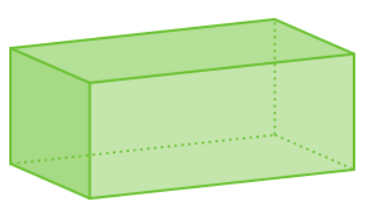
\includegraphics[width=0.4\linewidth]{figs/top-ov-box.png}
\\~\\
\end{center}
where the left and right sides are squares. What is the maximum volume your box can have?



\smallskip 

{\small \textit{Hint:  Be prepared to do some geometry first. Take one of the non-square sides and denote its length and width by $x$ and $y$. Can you express $y$ by $x$? Can you also express the volume by $x$?}
    }


\end{problem}



\medskip

\begin{problem}
    Calculate $\displaystyle \int f(x)\, dx$:
    \begin{enumerate}
        \item[a) ] $f(x)=3x^2$
        \item[b) ] $f(x)=x+6\cos x$
        \item[c) ] $f(x)=\dfrac{3}{x}-1$
        \item[d) ] $f(x)=\dfrac{4x}{1-2x^2}$
        % \item[e) ] $f(x)=\dfrac{2x}{1-x^2}$,
        \item[e) ] $f(x)=\text{tg}\,x$
    \end{enumerate}
\end{problem}

\medskip



\begin{problem}
The speed of a spaceship  at time $x$, as it flies from Earth to the Moon, is given by \[f(x) = x^5-x^2\] 
thousand kilometers per hour.
    \begin{enumerate}
        \item[a) ] How much distance does it pass in the first $3$ hours?

        \item[b) ] Consequently, how much was its average speed?  
    \end{enumerate}
\end{problem}

\medskip


\begin{problem}[\textbf{additional}]
Here the graph of the function $$f(x) = -x \cdot \ln (x^2)$$ 
on the interval $0 < x < 1$ is plotted:
\begin{center}
\\~\\
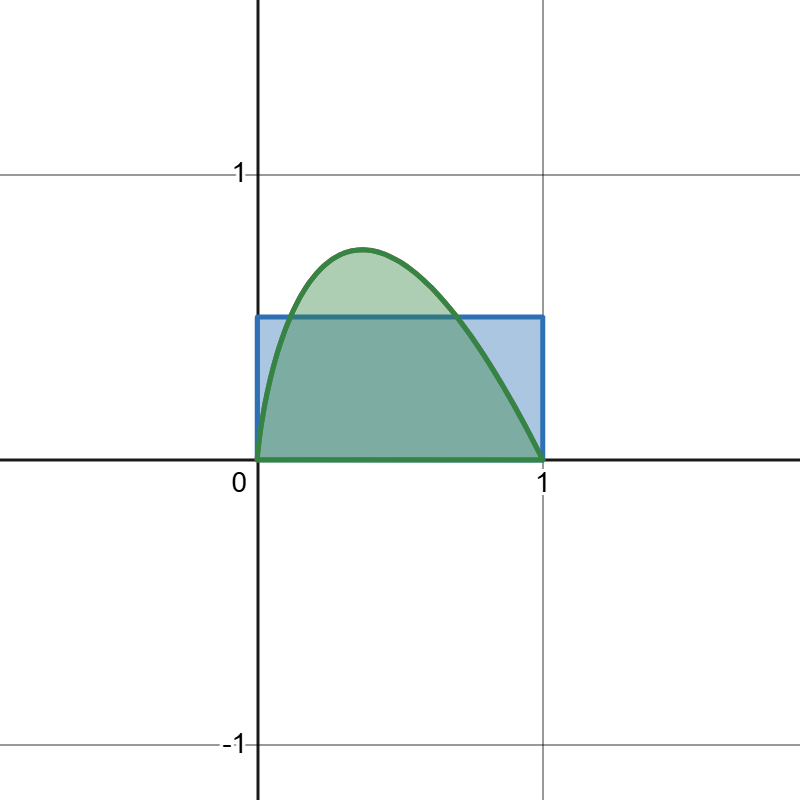
\includegraphics[width=0.5\linewidth]{figs/equal_areas.png}
\\~\\
\end{center}
It is known that the area of the green and blue regions  are the same. What is the height of the blue rectangle?

    
\end{problem}

% \medskip


% \begin{problem}[\textbf{additional++}]
% There are a couple of ways to make one new function from two given functions. One of them is \textit{convolution} which is a very  important technique in Machine Learning.

% Given two functions $f$ and $g$,  their convolution is a new function $f*g$, which is defined by the formula:
% \[
% (f*g)(x) = \int_{-1}^1 f(y)g(x-y) \, dy
% \]
% Given $f(x)=x^2$ and $g(x) = x^2$


    
% \end{problem}

% \bigskip

% \begin{problem}%[\textbf{optional, not graded}]
% Match the graphs 1-4 to functions i-iv: 
% \\~\\
% 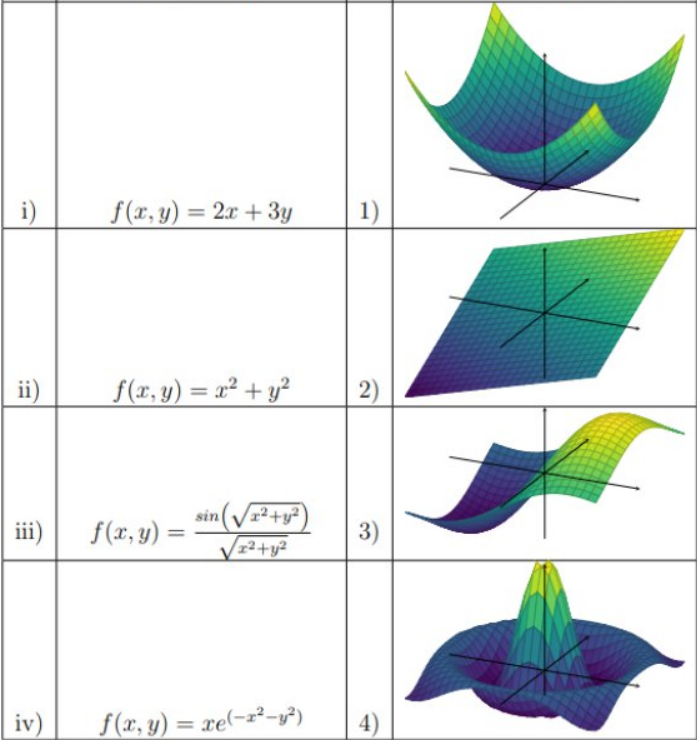
\includegraphics[width=0.6\linewidth]{figs/f(x,y) functions.png}
% \\~\\
% \end{problem}

% \bigskip
        
        